\documentclass{article} % For LaTeX2e
\usepackage{iclr2022_conference,times}
% Optional math commands from https://github.com/goodfeli/dlbook_notation.
%%%%% NEW MATH DEFINITIONS %%%%%

\usepackage{amsmath,amsfonts,bm}

% Mark sections of captions for referring to divisions of figures
\newcommand{\figleft}{{\em (Left)}}
\newcommand{\figcenter}{{\em (Center)}}
\newcommand{\figright}{{\em (Right)}}
\newcommand{\figtop}{{\em (Top)}}
\newcommand{\figbottom}{{\em (Bottom)}}
\newcommand{\captiona}{{\em (a)}}
\newcommand{\captionb}{{\em (b)}}
\newcommand{\captionc}{{\em (c)}}
\newcommand{\captiond}{{\em (d)}}

% Highlight a newly defined term
\newcommand{\newterm}[1]{{\bf #1}}


% Figure reference, lower-case.
\def\figref#1{figure~\ref{#1}}
% Figure reference, capital. For start of sentence
\def\Figref#1{Figure~\ref{#1}}
\def\twofigref#1#2{figures \ref{#1} and \ref{#2}}
\def\quadfigref#1#2#3#4{figures \ref{#1}, \ref{#2}, \ref{#3} and \ref{#4}}
% Section reference, lower-case.
\def\secref#1{section~\ref{#1}}
% Section reference, capital.
\def\Secref#1{Section~\ref{#1}}
% Reference to two sections.
\def\twosecrefs#1#2{sections \ref{#1} and \ref{#2}}
% Reference to three sections.
\def\secrefs#1#2#3{sections \ref{#1}, \ref{#2} and \ref{#3}}
% Reference to an equation, lower-case.
\def\eqref#1{equation~\ref{#1}}
% Reference to an equation, upper case
\def\Eqref#1{Equation~\ref{#1}}
% A raw reference to an equation---avoid using if possible
\def\plaineqref#1{\ref{#1}}
% Reference to a chapter, lower-case.
\def\chapref#1{chapter~\ref{#1}}
% Reference to an equation, upper case.
\def\Chapref#1{Chapter~\ref{#1}}
% Reference to a range of chapters
\def\rangechapref#1#2{chapters\ref{#1}--\ref{#2}}
% Reference to an algorithm, lower-case.
\def\algref#1{algorithm~\ref{#1}}
% Reference to an algorithm, upper case.
\def\Algref#1{Algorithm~\ref{#1}}
\def\twoalgref#1#2{algorithms \ref{#1} and \ref{#2}}
\def\Twoalgref#1#2{Algorithms \ref{#1} and \ref{#2}}
% Reference to a part, lower case
\def\partref#1{part~\ref{#1}}
% Reference to a part, upper case
\def\Partref#1{Part~\ref{#1}}
\def\twopartref#1#2{parts \ref{#1} and \ref{#2}}

\def\ceil#1{\lceil #1 \rceil}
\def\floor#1{\lfloor #1 \rfloor}
\def\1{\bm{1}}
\newcommand{\train}{\mathcal{D}}
\newcommand{\valid}{\mathcal{D_{\mathrm{valid}}}}
\newcommand{\test}{\mathcal{D_{\mathrm{test}}}}

\def\eps{{\epsilon}}


% Random variables
\def\reta{{\textnormal{$\eta$}}}
\def\ra{{\textnormal{a}}}
\def\rb{{\textnormal{b}}}
\def\rc{{\textnormal{c}}}
\def\rd{{\textnormal{d}}}
\def\re{{\textnormal{e}}}
\def\rf{{\textnormal{f}}}
\def\rg{{\textnormal{g}}}
\def\rh{{\textnormal{h}}}
\def\ri{{\textnormal{i}}}
\def\rj{{\textnormal{j}}}
\def\rk{{\textnormal{k}}}
\def\rl{{\textnormal{l}}}
% rm is already a command, just don't name any random variables m
\def\rn{{\textnormal{n}}}
\def\ro{{\textnormal{o}}}
\def\rp{{\textnormal{p}}}
\def\rq{{\textnormal{q}}}
\def\rr{{\textnormal{r}}}
\def\rs{{\textnormal{s}}}
\def\rt{{\textnormal{t}}}
\def\ru{{\textnormal{u}}}
\def\rv{{\textnormal{v}}}
\def\rw{{\textnormal{w}}}
\def\rx{{\textnormal{x}}}
\def\ry{{\textnormal{y}}}
\def\rz{{\textnormal{z}}}

% Random vectors
\def\rvepsilon{{\mathbf{\epsilon}}}
\def\rvtheta{{\mathbf{\theta}}}
\def\rva{{\mathbf{a}}}
\def\rvb{{\mathbf{b}}}
\def\rvc{{\mathbf{c}}}
\def\rvd{{\mathbf{d}}}
\def\rve{{\mathbf{e}}}
\def\rvf{{\mathbf{f}}}
\def\rvg{{\mathbf{g}}}
\def\rvh{{\mathbf{h}}}
\def\rvu{{\mathbf{i}}}
\def\rvj{{\mathbf{j}}}
\def\rvk{{\mathbf{k}}}
\def\rvl{{\mathbf{l}}}
\def\rvm{{\mathbf{m}}}
\def\rvn{{\mathbf{n}}}
\def\rvo{{\mathbf{o}}}
\def\rvp{{\mathbf{p}}}
\def\rvq{{\mathbf{q}}}
\def\rvr{{\mathbf{r}}}
\def\rvs{{\mathbf{s}}}
\def\rvt{{\mathbf{t}}}
\def\rvu{{\mathbf{u}}}
\def\rvv{{\mathbf{v}}}
\def\rvw{{\mathbf{w}}}
\def\rvx{{\mathbf{x}}}
\def\rvy{{\mathbf{y}}}
\def\rvz{{\mathbf{z}}}

% Elements of random vectors
\def\erva{{\textnormal{a}}}
\def\ervb{{\textnormal{b}}}
\def\ervc{{\textnormal{c}}}
\def\ervd{{\textnormal{d}}}
\def\erve{{\textnormal{e}}}
\def\ervf{{\textnormal{f}}}
\def\ervg{{\textnormal{g}}}
\def\ervh{{\textnormal{h}}}
\def\ervi{{\textnormal{i}}}
\def\ervj{{\textnormal{j}}}
\def\ervk{{\textnormal{k}}}
\def\ervl{{\textnormal{l}}}
\def\ervm{{\textnormal{m}}}
\def\ervn{{\textnormal{n}}}
\def\ervo{{\textnormal{o}}}
\def\ervp{{\textnormal{p}}}
\def\ervq{{\textnormal{q}}}
\def\ervr{{\textnormal{r}}}
\def\ervs{{\textnormal{s}}}
\def\ervt{{\textnormal{t}}}
\def\ervu{{\textnormal{u}}}
\def\ervv{{\textnormal{v}}}
\def\ervw{{\textnormal{w}}}
\def\ervx{{\textnormal{x}}}
\def\ervy{{\textnormal{y}}}
\def\ervz{{\textnormal{z}}}

% Random matrices
\def\rmA{{\mathbf{A}}}
\def\rmB{{\mathbf{B}}}
\def\rmC{{\mathbf{C}}}
\def\rmD{{\mathbf{D}}}
\def\rmE{{\mathbf{E}}}
\def\rmF{{\mathbf{F}}}
\def\rmG{{\mathbf{G}}}
\def\rmH{{\mathbf{H}}}
\def\rmI{{\mathbf{I}}}
\def\rmJ{{\mathbf{J}}}
\def\rmK{{\mathbf{K}}}
\def\rmL{{\mathbf{L}}}
\def\rmM{{\mathbf{M}}}
\def\rmN{{\mathbf{N}}}
\def\rmO{{\mathbf{O}}}
\def\rmP{{\mathbf{P}}}
\def\rmQ{{\mathbf{Q}}}
\def\rmR{{\mathbf{R}}}
\def\rmS{{\mathbf{S}}}
\def\rmT{{\mathbf{T}}}
\def\rmU{{\mathbf{U}}}
\def\rmV{{\mathbf{V}}}
\def\rmW{{\mathbf{W}}}
\def\rmX{{\mathbf{X}}}
\def\rmY{{\mathbf{Y}}}
\def\rmZ{{\mathbf{Z}}}

% Elements of random matrices
\def\ermA{{\textnormal{A}}}
\def\ermB{{\textnormal{B}}}
\def\ermC{{\textnormal{C}}}
\def\ermD{{\textnormal{D}}}
\def\ermE{{\textnormal{E}}}
\def\ermF{{\textnormal{F}}}
\def\ermG{{\textnormal{G}}}
\def\ermH{{\textnormal{H}}}
\def\ermI{{\textnormal{I}}}
\def\ermJ{{\textnormal{J}}}
\def\ermK{{\textnormal{K}}}
\def\ermL{{\textnormal{L}}}
\def\ermM{{\textnormal{M}}}
\def\ermN{{\textnormal{N}}}
\def\ermO{{\textnormal{O}}}
\def\ermP{{\textnormal{P}}}
\def\ermQ{{\textnormal{Q}}}
\def\ermR{{\textnormal{R}}}
\def\ermS{{\textnormal{S}}}
\def\ermT{{\textnormal{T}}}
\def\ermU{{\textnormal{U}}}
\def\ermV{{\textnormal{V}}}
\def\ermW{{\textnormal{W}}}
\def\ermX{{\textnormal{X}}}
\def\ermY{{\textnormal{Y}}}
\def\ermZ{{\textnormal{Z}}}

% Vectors
\def\vzero{{\bm{0}}}
\def\vone{{\bm{1}}}
\def\vmu{{\bm{\mu}}}
\def\vtheta{{\bm{\theta}}}
\def\va{{\bm{a}}}
\def\vb{{\bm{b}}}
\def\vc{{\bm{c}}}
\def\vd{{\bm{d}}}
\def\ve{{\bm{e}}}
\def\vf{{\bm{f}}}
\def\vg{{\bm{g}}}
\def\vh{{\bm{h}}}
\def\vi{{\bm{i}}}
\def\vj{{\bm{j}}}
\def\vk{{\bm{k}}}
\def\vl{{\bm{l}}}
\def\vm{{\bm{m}}}
\def\vn{{\bm{n}}}
\def\vo{{\bm{o}}}
\def\vp{{\bm{p}}}
\def\vq{{\bm{q}}}
\def\vr{{\bm{r}}}
\def\vs{{\bm{s}}}
\def\vt{{\bm{t}}}
\def\vu{{\bm{u}}}
\def\vv{{\bm{v}}}
\def\vw{{\bm{w}}}
\def\vx{{\bm{x}}}
\def\vy{{\bm{y}}}
\def\vz{{\bm{z}}}

% Elements of vectors
\def\evalpha{{\alpha}}
\def\evbeta{{\beta}}
\def\evepsilon{{\epsilon}}
\def\evlambda{{\lambda}}
\def\evomega{{\omega}}
\def\evmu{{\mu}}
\def\evpsi{{\psi}}
\def\evsigma{{\sigma}}
\def\evtheta{{\theta}}
\def\eva{{a}}
\def\evb{{b}}
\def\evc{{c}}
\def\evd{{d}}
\def\eve{{e}}
\def\evf{{f}}
\def\evg{{g}}
\def\evh{{h}}
\def\evi{{i}}
\def\evj{{j}}
\def\evk{{k}}
\def\evl{{l}}
\def\evm{{m}}
\def\evn{{n}}
\def\evo{{o}}
\def\evp{{p}}
\def\evq{{q}}
\def\evr{{r}}
\def\evs{{s}}
\def\evt{{t}}
\def\evu{{u}}
\def\evv{{v}}
\def\evw{{w}}
\def\evx{{x}}
\def\evy{{y}}
\def\evz{{z}}

% Matrix
\def\mA{{\bm{A}}}
\def\mB{{\bm{B}}}
\def\mC{{\bm{C}}}
\def\mD{{\bm{D}}}
\def\mE{{\bm{E}}}
\def\mF{{\bm{F}}}
\def\mG{{\bm{G}}}
\def\mH{{\bm{H}}}
\def\mI{{\bm{I}}}
\def\mJ{{\bm{J}}}
\def\mK{{\bm{K}}}
\def\mL{{\bm{L}}}
\def\mM{{\bm{M}}}
\def\mN{{\bm{N}}}
\def\mO{{\bm{O}}}
\def\mP{{\bm{P}}}
\def\mQ{{\bm{Q}}}
\def\mR{{\bm{R}}}
\def\mS{{\bm{S}}}
\def\mT{{\bm{T}}}
\def\mU{{\bm{U}}}
\def\mV{{\bm{V}}}
\def\mW{{\bm{W}}}
\def\mX{{\bm{X}}}
\def\mY{{\bm{Y}}}
\def\mZ{{\bm{Z}}}
\def\mBeta{{\bm{\beta}}}
\def\mPhi{{\bm{\Phi}}}
\def\mLambda{{\bm{\Lambda}}}
\def\mSigma{{\bm{\Sigma}}}

% Tensor
\DeclareMathAlphabet{\mathsfit}{\encodingdefault}{\sfdefault}{m}{sl}
\SetMathAlphabet{\mathsfit}{bold}{\encodingdefault}{\sfdefault}{bx}{n}
\newcommand{\tens}[1]{\bm{\mathsfit{#1}}}
\def\tA{{\tens{A}}}
\def\tB{{\tens{B}}}
\def\tC{{\tens{C}}}
\def\tD{{\tens{D}}}
\def\tE{{\tens{E}}}
\def\tF{{\tens{F}}}
\def\tG{{\tens{G}}}
\def\tH{{\tens{H}}}
\def\tI{{\tens{I}}}
\def\tJ{{\tens{J}}}
\def\tK{{\tens{K}}}
\def\tL{{\tens{L}}}
\def\tM{{\tens{M}}}
\def\tN{{\tens{N}}}
\def\tO{{\tens{O}}}
\def\tP{{\tens{P}}}
\def\tQ{{\tens{Q}}}
\def\tR{{\tens{R}}}
\def\tS{{\tens{S}}}
\def\tT{{\tens{T}}}
\def\tU{{\tens{U}}}
\def\tV{{\tens{V}}}
\def\tW{{\tens{W}}}
\def\tX{{\tens{X}}}
\def\tY{{\tens{Y}}}
\def\tZ{{\tens{Z}}}


% Graph
\def\gA{{\mathcal{A}}}
\def\gB{{\mathcal{B}}}
\def\gC{{\mathcal{C}}}
\def\gD{{\mathcal{D}}}
\def\gE{{\mathcal{E}}}
\def\gF{{\mathcal{F}}}
\def\gG{{\mathcal{G}}}
\def\gH{{\mathcal{H}}}
\def\gI{{\mathcal{I}}}
\def\gJ{{\mathcal{J}}}
\def\gK{{\mathcal{K}}}
\def\gL{{\mathcal{L}}}
\def\gM{{\mathcal{M}}}
\def\gN{{\mathcal{N}}}
\def\gO{{\mathcal{O}}}
\def\gP{{\mathcal{P}}}
\def\gQ{{\mathcal{Q}}}
\def\gR{{\mathcal{R}}}
\def\gS{{\mathcal{S}}}
\def\gT{{\mathcal{T}}}
\def\gU{{\mathcal{U}}}
\def\gV{{\mathcal{V}}}
\def\gW{{\mathcal{W}}}
\def\gX{{\mathcal{X}}}
\def\gY{{\mathcal{Y}}}
\def\gZ{{\mathcal{Z}}}

% Sets
\def\sA{{\mathbb{A}}}
\def\sB{{\mathbb{B}}}
\def\sC{{\mathbb{C}}}
\def\sD{{\mathbb{D}}}
% Don't use a set called E, because this would be the same as our symbol
% for expectation.
\def\sF{{\mathbb{F}}}
\def\sG{{\mathbb{G}}}
\def\sH{{\mathbb{H}}}
\def\sI{{\mathbb{I}}}
\def\sJ{{\mathbb{J}}}
\def\sK{{\mathbb{K}}}
\def\sL{{\mathbb{L}}}
\def\sM{{\mathbb{M}}}
\def\sN{{\mathbb{N}}}
\def\sO{{\mathbb{O}}}
\def\sP{{\mathbb{P}}}
\def\sQ{{\mathbb{Q}}}
\def\sR{{\mathbb{R}}}
\def\sS{{\mathbb{S}}}
\def\sT{{\mathbb{T}}}
\def\sU{{\mathbb{U}}}
\def\sV{{\mathbb{V}}}
\def\sW{{\mathbb{W}}}
\def\sX{{\mathbb{X}}}
\def\sY{{\mathbb{Y}}}
\def\sZ{{\mathbb{Z}}}

% Entries of a matrix
\def\emLambda{{\Lambda}}
\def\emA{{A}}
\def\emB{{B}}
\def\emC{{C}}
\def\emD{{D}}
\def\emE{{E}}
\def\emF{{F}}
\def\emG{{G}}
\def\emH{{H}}
\def\emI{{I}}
\def\emJ{{J}}
\def\emK{{K}}
\def\emL{{L}}
\def\emM{{M}}
\def\emN{{N}}
\def\emO{{O}}
\def\emP{{P}}
\def\emQ{{Q}}
\def\emR{{R}}
\def\emS{{S}}
\def\emT{{T}}
\def\emU{{U}}
\def\emV{{V}}
\def\emW{{W}}
\def\emX{{X}}
\def\emY{{Y}}
\def\emZ{{Z}}
\def\emSigma{{\Sigma}}

% entries of a tensor
% Same font as tensor, without \bm wrapper
\newcommand{\etens}[1]{\mathsfit{#1}}
\def\etLambda{{\etens{\Lambda}}}
\def\etA{{\etens{A}}}
\def\etB{{\etens{B}}}
\def\etC{{\etens{C}}}
\def\etD{{\etens{D}}}
\def\etE{{\etens{E}}}
\def\etF{{\etens{F}}}
\def\etG{{\etens{G}}}
\def\etH{{\etens{H}}}
\def\etI{{\etens{I}}}
\def\etJ{{\etens{J}}}
\def\etK{{\etens{K}}}
\def\etL{{\etens{L}}}
\def\etM{{\etens{M}}}
\def\etN{{\etens{N}}}
\def\etO{{\etens{O}}}
\def\etP{{\etens{P}}}
\def\etQ{{\etens{Q}}}
\def\etR{{\etens{R}}}
\def\etS{{\etens{S}}}
\def\etT{{\etens{T}}}
\def\etU{{\etens{U}}}
\def\etV{{\etens{V}}}
\def\etW{{\etens{W}}}
\def\etX{{\etens{X}}}
\def\etY{{\etens{Y}}}
\def\etZ{{\etens{Z}}}

% The true underlying data generating distribution
\newcommand{\pdata}{p_{\rm{data}}}
% The empirical distribution defined by the training set
\newcommand{\ptrain}{\hat{p}_{\rm{data}}}
\newcommand{\Ptrain}{\hat{P}_{\rm{data}}}
% The model distribution
\newcommand{\pmodel}{p_{\rm{model}}}
\newcommand{\Pmodel}{P_{\rm{model}}}
\newcommand{\ptildemodel}{\tilde{p}_{\rm{model}}}
% Stochastic autoencoder distributions
\newcommand{\pencode}{p_{\rm{encoder}}}
\newcommand{\pdecode}{p_{\rm{decoder}}}
\newcommand{\precons}{p_{\rm{reconstruct}}}

\newcommand{\laplace}{\mathrm{Laplace}} % Laplace distribution

\newcommand{\E}{\mathbb{E}}
\newcommand{\Ls}{\mathcal{L}}
\newcommand{\R}{\mathbb{R}}
\newcommand{\emp}{\tilde{p}}
\newcommand{\lr}{\alpha}
\newcommand{\reg}{\lambda}
\newcommand{\rect}{\mathrm{rectifier}}
\newcommand{\softmax}{\mathrm{softmax}}
\newcommand{\sigmoid}{\sigma}
\newcommand{\softplus}{\zeta}
\newcommand{\KL}{D_{\mathrm{KL}}}
\newcommand{\Var}{\mathrm{Var}}
\newcommand{\standarderror}{\mathrm{SE}}
\newcommand{\Cov}{\mathrm{Cov}}
% Wolfram Mathworld says $L^2$ is for function spaces and $\ell^2$ is for vectors
% But then they seem to use $L^2$ for vectors throughout the site, and so does
% wikipedia.
\newcommand{\normlzero}{L^0}
\newcommand{\normlone}{L^1}
\newcommand{\normltwo}{L^2}
\newcommand{\normlp}{L^p}
\newcommand{\normmax}{L^\infty}

\newcommand{\parents}{Pa} % See usage in notation.tex. Chosen to match Daphne's book.

\DeclareMathOperator*{\argmax}{arg\,max}
\DeclareMathOperator*{\argmin}{arg\,min}

\DeclareMathOperator{\sign}{sign}
\DeclareMathOperator{\Tr}{Tr}
\let\ab\allowbreak


%######## APS360: Uncomment your submission name
%\newcommand{\apsname}{Project Proposal}
\newcommand{\apsname}{Progress Report}
%\newcommand{\apsname}{Final Report}

%######## APS360: Put your Group Number here
\newcommand{\gpnumber}{33}

\usepackage{hyperref}
\usepackage{url}
\usepackage{graphicx}
\usepackage{booktabs}
\usepackage{multirow}
\usepackage{tabularx}
\usepackage{float}

%######## APS360: Put your project Title here
\title{Skin Disease Detection Progres Report}

%######## APS360: Put your names, student IDs and Emails here
\author{Jacky Li  \\
Student\# 1011271678\\
\texttt{jakkii.li@mail.utoronto.ca} \\
\And
Jordan Cui  \\
Student\# 1011026916 \\
\texttt{jordan.cui@mail.utoronto.ca \phantom{    }} \\
\AND
Lawrence Ding  \\
Student\# 1011439025 \\
\texttt{larryzm.ding@mail.utoronto.ca} \\
\And
Soham Shorey \\
Student\# 1010845169 \\
\texttt{soham.shorey@mail.utoronto.ca} \\
\AND
}

\newcommand{\fix}{\marginpar{FIX}}
\newcommand{\new}{\marginpar{NEW}}

\iclrfinalcopy 
%######## APS360: Document starts here
\begin{document}

\maketitle

\vspace{-1cm}

\begin{abstract}
This report outlines our progress on developing a deep-learning based system to classify dermatological conditions from skin images. We aim to create a diagnostic tool that allows patients to detect potentially severe skin conditions early and aids healthcare professionals in diagnosis. It includes our individual contributions to the project and our delegated next tasks to complete our project on time. We have combined the HAM10000, BCN20000, and PAD-UFES-20 datasets with 9 standardized class labels. For reference, we trained a baseline KNN model with a ResNet-18 feature embedder achieving a 56.3\% accuracy. Our best current CNN classifier uses a ResNet-34 feature embedder backbone with a custom linear classifier to achieve 81.9\% accuracy. We outline the training strategies, hyperparameters, and architecture we used to train the model, and potential future improvements in data preprocessing and model architecture.
%######## APS360: Do not change the next line. This shows your Main body page count.
----Total Pages: \pageref{last_page}
\end{abstract}

\section{Brief Project Description}

Our team is developing a deep learning model to detect and classify common and rare skin conditions from dermoscopic and clinical images. The project focuses on distinguishing between various harmful and harmless skin conditions including nevus, melanoma, keratosis, basal cell carcinoma, squamous cell carcinoma, and other dermatological conditions to assist both patients and healthcare professionals in early detection and diagnosis.

The motivation behind our project is the fact that skin conditions affect over a third of the global population \citep{li2024epidemiological}. In Canada, 20\% of people experience acne, 1 million have psoriasis, and melanoma rates have risen by over 2\% annually since the 1980s \citep{canadian_dermatology_association}. In 2013, 84 million Americans, or a quarter of their population, saw a doctor for skin issues \citep{american_academy_dermatology}. A tool that classifies skin diseases from images could ease the burden on dermatologic healthcare by supporting early detection and aiding diagnosis.

\begin{figure}[h]
\begin{center}
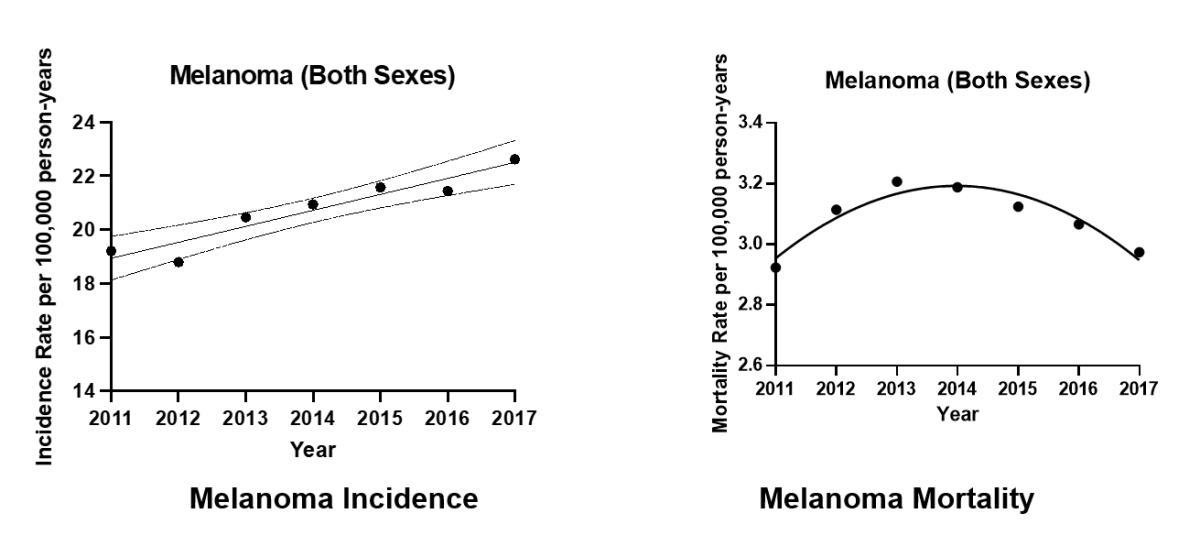
\includegraphics[width=0.55\textwidth]{Figs/melanoma_incidence_mortality.png}
\end{center}
\caption{Melanoma Incidence and Mortality Rate per 100,000 persons-year vs. Year \citep{mcgill_melanoma}.}
\end{figure}

Figure 1 demonstrates that the incidence of melanoma has been increasing steadily each year; however, it also shows that the mortality rate is decreasing relative to the incidence rate, likely due to advances in treatment techniques. This suggests that early diagnosis of melanoma is critical, as the disease is becoming more prevalent while also more treatable when caught early. These trends motivate us to build a disease detection tool to help individuals identify potential signs of melanoma sooner, encouraging timely medical attention and reducing the risk of severe outcomes.

The goal of our project is to create an automated skin disease detection system that can provide preliminary screening for various skin conditions, assist healthcare professionals in diagnostic decision-making, encourage timely medical consultation for potentially serious conditions, and ultimately reduce the burden on healthcare systems. The system takes dermoscopic images as input and outputs predicted skin disease classifications along with recommended next steps for patients.

\begin{figure}[h]
\begin{center}
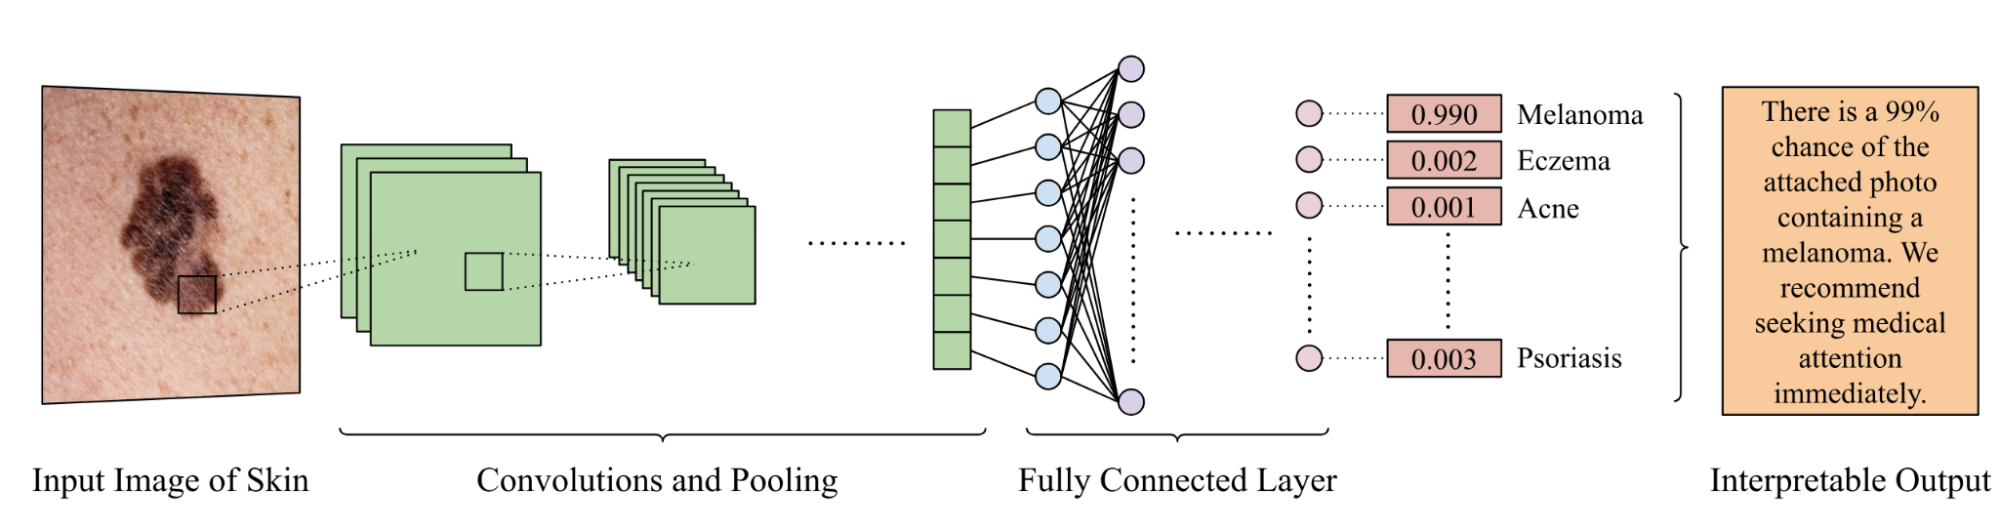
\includegraphics[width=0.7\textwidth]{Figs/system_visualization.png}
\end{center}
\caption{Visualization of the Proposed Model Architecture with Input and Output. The use of CNNs can be inferred from the figure.}
\end{figure}

Deep learning models, particularly convolutional neural networks (CNNs), are the most appropriate approach for this image classification task. CNNs use trainable filters to extract high-level spatial patterns in images. The use of shared weights also increases the computational efficiency of CNNs compared to fully connected alternatives. Since skin disease detection requires processing large amounts of image data, learning complex visual patterns where subtle differences can affect diagnosis, and using datasets with expert-labelled diseases, using a CNN model trained via supervised learning would yield the most effective classifier.

Lastly, we find this project interesting because it lies at the intersection of biomedical and machine learning engineering, two fields we are both passionate about and hope to explore further. Once completed, we plan to deploy the system as a publicly accessible web application. This will allow medical professionals to test the prototype in real-world settings and provide feedback, while also offering individuals without a diagnosis a chance to perform an initial screening of their skin condition. By making the tool accessible, we hope to raise awareness about early detection, improve access to preliminary assessment, and ultimately contribute to better health outcomes through the responsible use of AI in healthcare.

\section{Individual Contributions and Responsibilities}

Our team collaborates through GitHub for code management, Discord for daily communication, and a shared Google Sheet to track tasks and deadlines. We hold regular meetings to review progress and assign new responsibilities, while maintaining continuous communication via Discord. Although tasks are assigned to specific individuals, team members frequently assist one another. This approach helps ensure timely completion and provides redundancy in case someone faces unforeseen challenges. The individual contributions and task assignments listed below reflect those on our Google Sheet; however, in practice, our work is highly collaborative and often overlaps beyond these formal assignments.

\textbf{Jacky Li}
\begin{itemize}
\item Established the GitHub repository and development workflow.
\item Led model research, including literature review on potential baseline models and transfer learning models like ResNet and EfficientNet for classifiers.
\item Developed and maintained the data splitting and augmentation scripts.
\item Next steps: Support integration and comparison of advanced model architectures; assist with final model selection and analysis.
\end{itemize}

\textbf{Soham Shorey}
\begin{itemize}
\item Led data collection and processing including downloading and organizing all datasets.
\item Developed and executed the data preprocessing pipeline, including label standardization and image resizing.
\item Generated dataset statistics and visualizations to assess class balance.
\item Implemented the primary model and performed initial evaluation.
\item Next steps: Update and finalize data visualizations; prepare cleaned data examples for the report; assist with model retraining as needed.
\end{itemize}

\textbf{Jordan Cui}
\begin{itemize}
\item Led the documentation and organization of results into this progress report.
\item Assisted in the implementation of the baseline model.
\item Added evaluation metrics and visualizations for model performance.
\item Next steps: Finalize model training scripts; update evaluation metrics; help compile results and figures for the final report.
\end{itemize}

\textbf{Lawrence Ding}
\begin{itemize}
\item Researched typical baseline models used for medical imaging.
\item Implemented the baseline model and performed initial evaluation.
\item Assisted with dataset integration and preprocessing optimization.
\item Supported model training, validation, and hyperparameter tuning.
\item Next steps: Prepare scripts for final testing on unseen data; analyze and summarize model results; contribute to the final report and presentation.
\end{itemize}

\begin{figure}[h]
\begin{center}
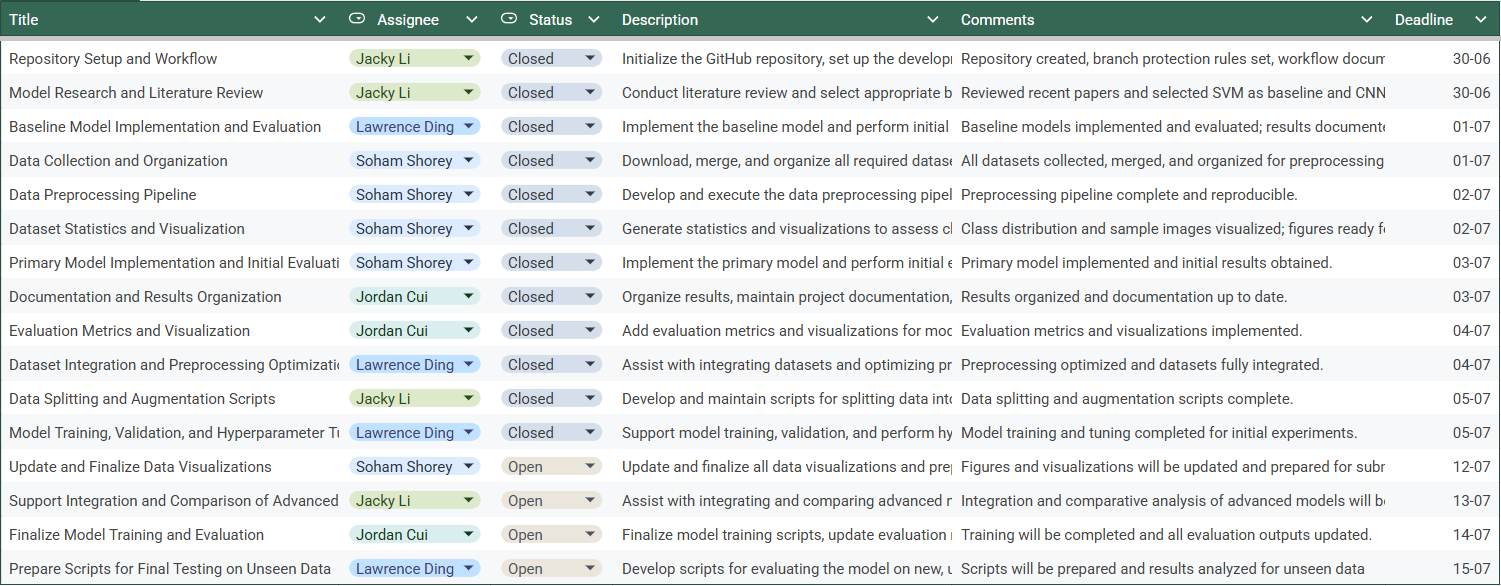
\includegraphics[width=0.8\textwidth]{Figs/google_sheet_tracking.png}
\end{center}
\caption{An image of the Google Sheet we used to track, assign, and efficiently take on tasks.}
\end{figure}

\section{Notable Contributions}

\subsection{Data Processing}

We combined three publicly available skin lesion datasets to create a comprehensive and diverse training set that offers robust coverage of various skin conditions and imaging modalities.

\subsubsection{Data Sources}

Our data was sourced from three datasets: BCN20000, HAM10000, and PAD-UFES-20.

\begin{itemize}
\item The BCN20000 dataset contains 18,946 dermoscopic images sourced from the Hospital Clínic de Barcelona corresponding to 8 skin conditions \citep{isic_bcn20000}. The dataset was sourced using the ISIC archive using a metadata CSV to extract only the BCN20000 images.
\item The HAM10000 dataset contains 10,015 dermatoscopic images from 7 different classes sourced from the Department of Dermatology at the Medical University of Vienna, Austria, and the skin cancer practice of Cliff Rosendahl in Queensland, Australia over 20 years \citep{ham10000_dataset}. The dataset was sourced from Kaggle and stored in 2 separate folders which were combined.
\item The PAD-UFES-20 dataset contains 2,298 labelled images of dermatological conditions sourced by the Federal University of Espírito Santo (UFES) in Brazil. The dataset was sourced from Kaggle, which required merging images from three separate folders into a unified directory structure \citep{pad_ufes_dataset}.
\end{itemize}

\subsubsection{Data Cleaning and Processing Steps}

The unification of these three datasets required multiple preprocessing steps.

Since the BCN20000 dataset is not publicly separated from the broader ISIC archive, we used a metadata CSV file to isolate and include only the BCN20000-labeled images. For the HAM10000 and PAD-UFES-20 datasets, we consolidated images from all respective folders into unified directory structures.

Label information was extracted from the diagnosis\_3 field in the BCN20000 metadata, the dx field in the HAM10000 metadata, and the diagnostic field in the PAD-UFES-20 CSV. We then standardized all labels into nine unified classes: nevus, melanoma, actinic (pre-cancerous) keratosis, basal cell carcinoma (BCC), squamous cell carcinoma (SCC), lentigo, vascular lesion, dermatofibroma, and keratosis.

\begin{figure}[h]
\begin{center}
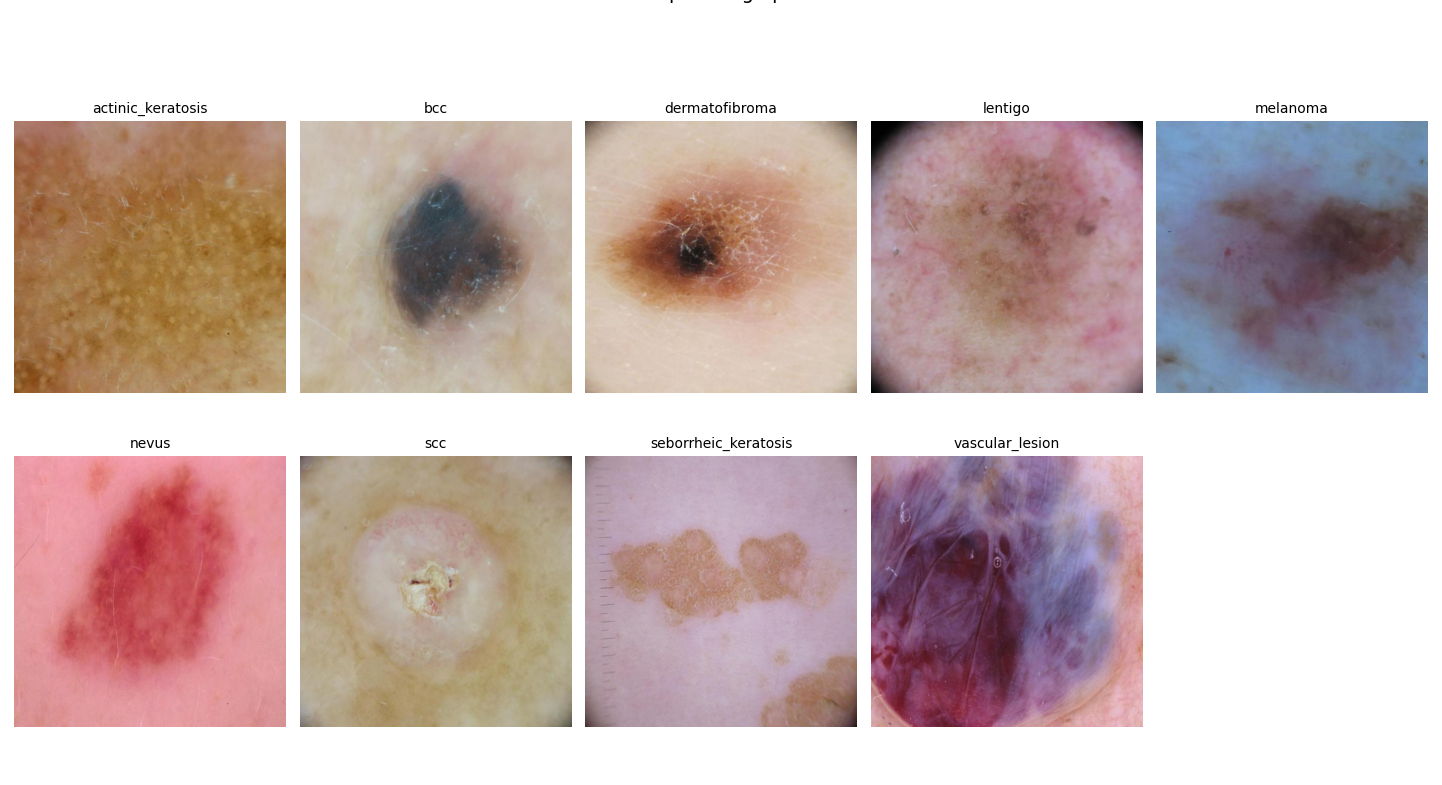
\includegraphics[width=0.6\textwidth]{Figs/sample_class_images.png}
\end{center}
\caption{Sample resized and labelled images from each of the 9 classes in the combined dataset.}
\end{figure}

We first used the ISIC API along with the BCN20000\_metadata.csv file to extract only the BCN20000 images. We downloaded the HAM10000 and PAD-UFES-20 datasets from Kaggle.

Before consolidation, we resized all images to 512 × 512 using the PIL.Image library for consistent input sizes. Then, we organized all files into unified directories based on standardized label categories. For example, images labelled nevi were mapped to the \textit{nevus} folder.

Approximately 1,000 images labeled as scars or left unlabeled were grouped under \textit{other} and excluded from training. We considered applying a hair removal filter to reduce skin image noise but decided to gauge model performance before its application \citep{kalpana2025enhancing}.

\begin{figure}[h]
\begin{center}
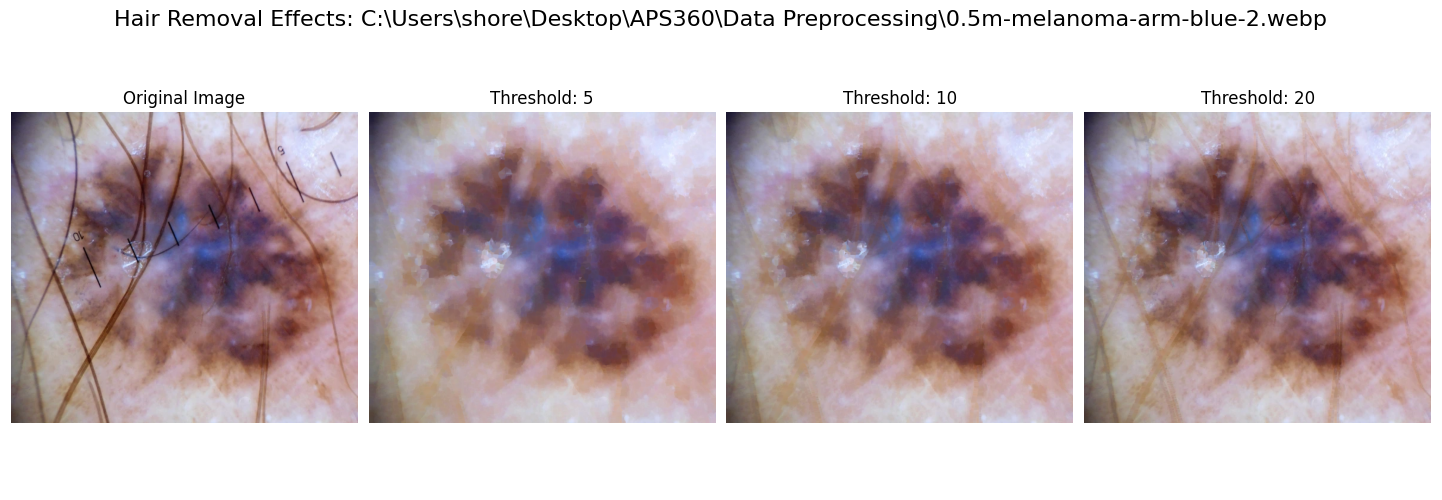
\includegraphics[width=0.6\textwidth]{Figs/hair_removal_filter.png}
\end{center}
\caption{Effect of hair removal filter at thresholds 5, 10, and 15 on sample melanoma image. Filter removes hair and measurement lines from the image.}
\end{figure}

\subsubsection{Dataset Statistics}

\begin{figure}[H]
\begin{center}
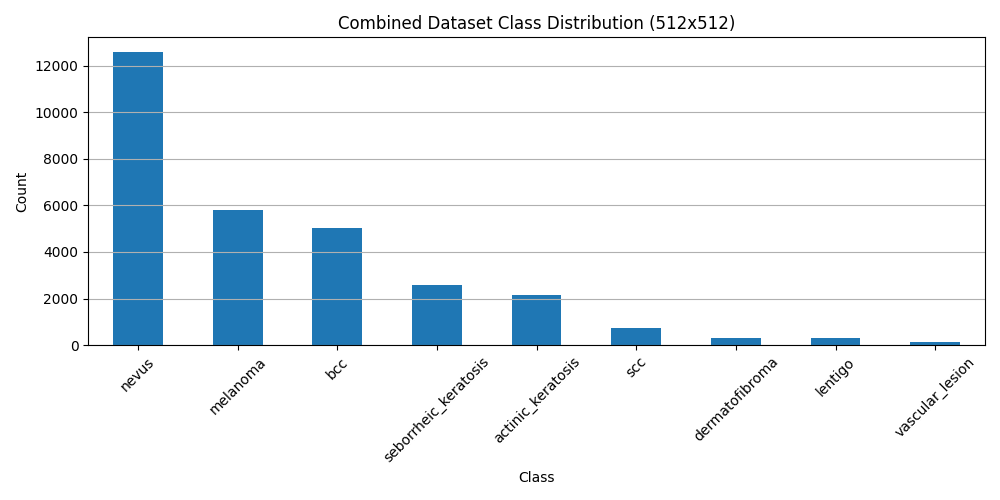
\includegraphics[width=0.8\textwidth]{Figs/class_distribution.png}
\end{center}
\caption{Class distribution of combined dataset, imbalanced with nevus as the majority class.}
\end{figure}

\begin{table}[h]
\caption{Class counts after preprocessing}
\label{class-counts}
\begin{center}
\footnotesize
\begin{tabular}{lccccc}
\toprule
\textbf{Class} & \textbf{Nevus} & \textbf{Melanoma} & \textbf{BCC} & \textbf{Benign keratosis} & \textbf{Actinic keratosis} \\
\textbf{Count} & 12,596 & 5,801 & 5,035 & 2,602 & 2,145 \\
\midrule
\textbf{Class} & \textbf{SCC} & \textbf{Dermatofibroma} & \textbf{Lentigo} & \textbf{Vascular lesions} & \\
\textbf{Count} & 751 & 283 & 283 & 142 & \\
\midrule
\multicolumn{6}{c}{\textbf{Total: 29,638}} \\
\bottomrule
\end{tabular}
\end{center}
\end{table}

\begin{figure}[H]
\begin{center}
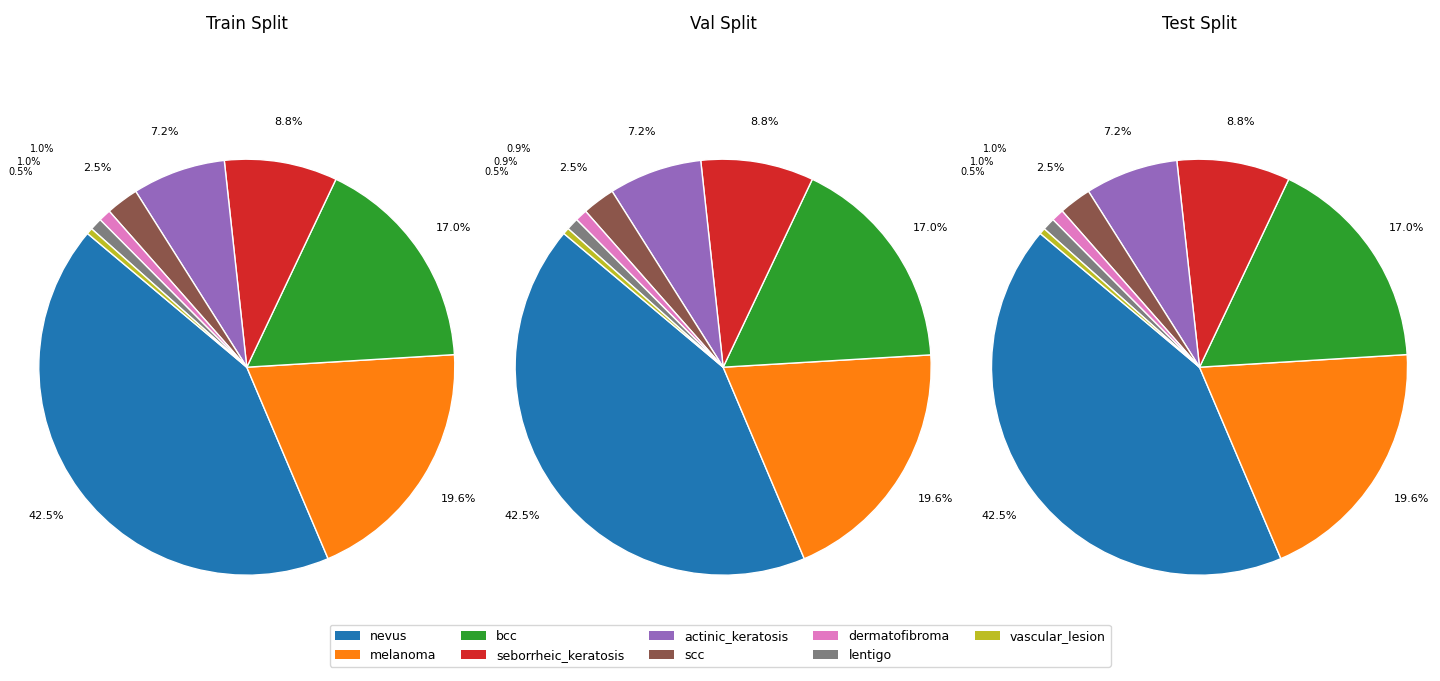
\includegraphics[width=0.7\textwidth]{Figs/dataset_split_distribution.png}
\end{center}
\caption{Even class distribution between training, validation, and testing datasets.}
\end{figure}

We split the processed dataset into 70\% training, 15\% validation, and 15\% test sets to ensure robust model training and evaluation. Each split maintains the same class distribution as visualized in the dataset summary above. However, the dataset remains significantly imbalanced, with the \textit{nevus} class accounting for approximately 42.5\% of all samples.

In the future, if the class imbalance remains an issue, we may add more samples of underrepresented classes using datasets like DERM12345 and reputable dermatological image sources like DermNet.

We created class distribution visualizations using matplotlib to identify label imbalances. These bar charts allow us to verify data quality and plan appropriate sampling and augmentation strategies for training.

\subsubsection{Challenges}

We encountered several significant challenges during data processing.

\begin{itemize}
\item Since HAM10000 and BCN20000 images are present in the ISIC challenge datasets, we identified duplicate images as a potential issue. To ensure neither dataset overlapped, we compared ISIC IDs of HAM10000 and BCN20000 images to ensure no duplicate images were present in our dataset.
\item BCN20000 images are not publicly available as a separate dataset. As such, BCN20000 images were extracted from the ISIC20000 dataset using a metadata CSV file.
\item Label inconsistencies between datasets required building a comprehensive mapping system to consolidate similar labels into unified classes.
\end{itemize}

\subsubsection{Plan for Final Testing on Unseen Data}

Our final model will be evaluated on the dedicated test data containing 4,446 images unseen by the model during training. We will also test our model on completely separate datasets like DERM12345 and Fitzpatrick17k if not previously used in our training process. Ideally, we aim to manually collect dermoscopic images from open sources or clinical repositories to ensure completely unseen test data to best evaluate the generalization capabilities of our model.

\subsection{Baseline Model}

\begin{figure}[H]
\begin{center}
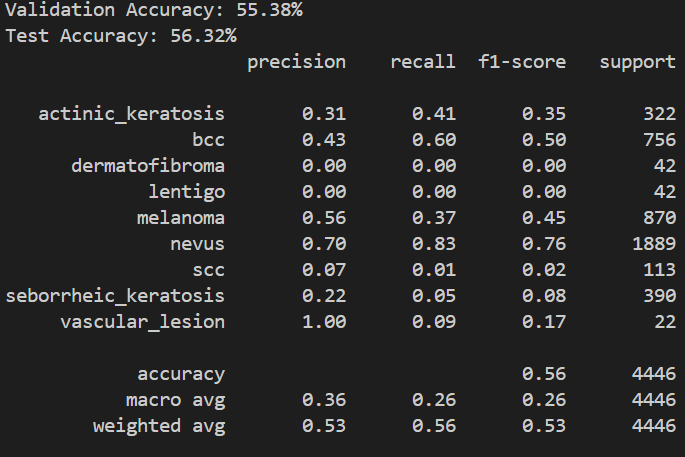
\includegraphics[width=0.6\textwidth]{Figs/baseline_performance.png}
\end{center}
\caption{Accuracy, precision, recall, and F1-score of the baseline model. This model struggles with the imbalanced dataset, with a high F1-score for the most common class, but completely fails at identifying the less common classes.}
\end{figure}


For our baseline model, we initially considered using simpler SVM or KNN algorithms to compare our model to. However, due to the complexity of skin detection, a standalone SVM or KNN is unlikely to outperform random chance. As such, we chose to first extract the features of the images using a pre-trained model (in this case the ResNet-18) and train a KNN model using the extracted features. In short, we imported the ResNet-18 and removed the fully-connected layers, only preserving the convolutional and average pool layers, and used it to extract the features of all the images in our dataset. The features were then used as data to fit a KNN model. The final test accuracy of this baseline model was only 56.32\% with the F1-scores not being acceptable for real-world applications. However, this model performs better than chance (11.11\%), and serves as a suitable baseline model for this project.


\subsection{Primary Model}

To develop an effective skin condition classifier, we tested several models with various CNN backbones, image transformations, classifier architectures, and model complexities. Each model leveraged transfer learning using ImageNet-pretrained feature extractors such as ResNet, EfficientNet, and MobileNet, combined with different custom classifier heads.

\begin{figure}[h]
\begin{center}
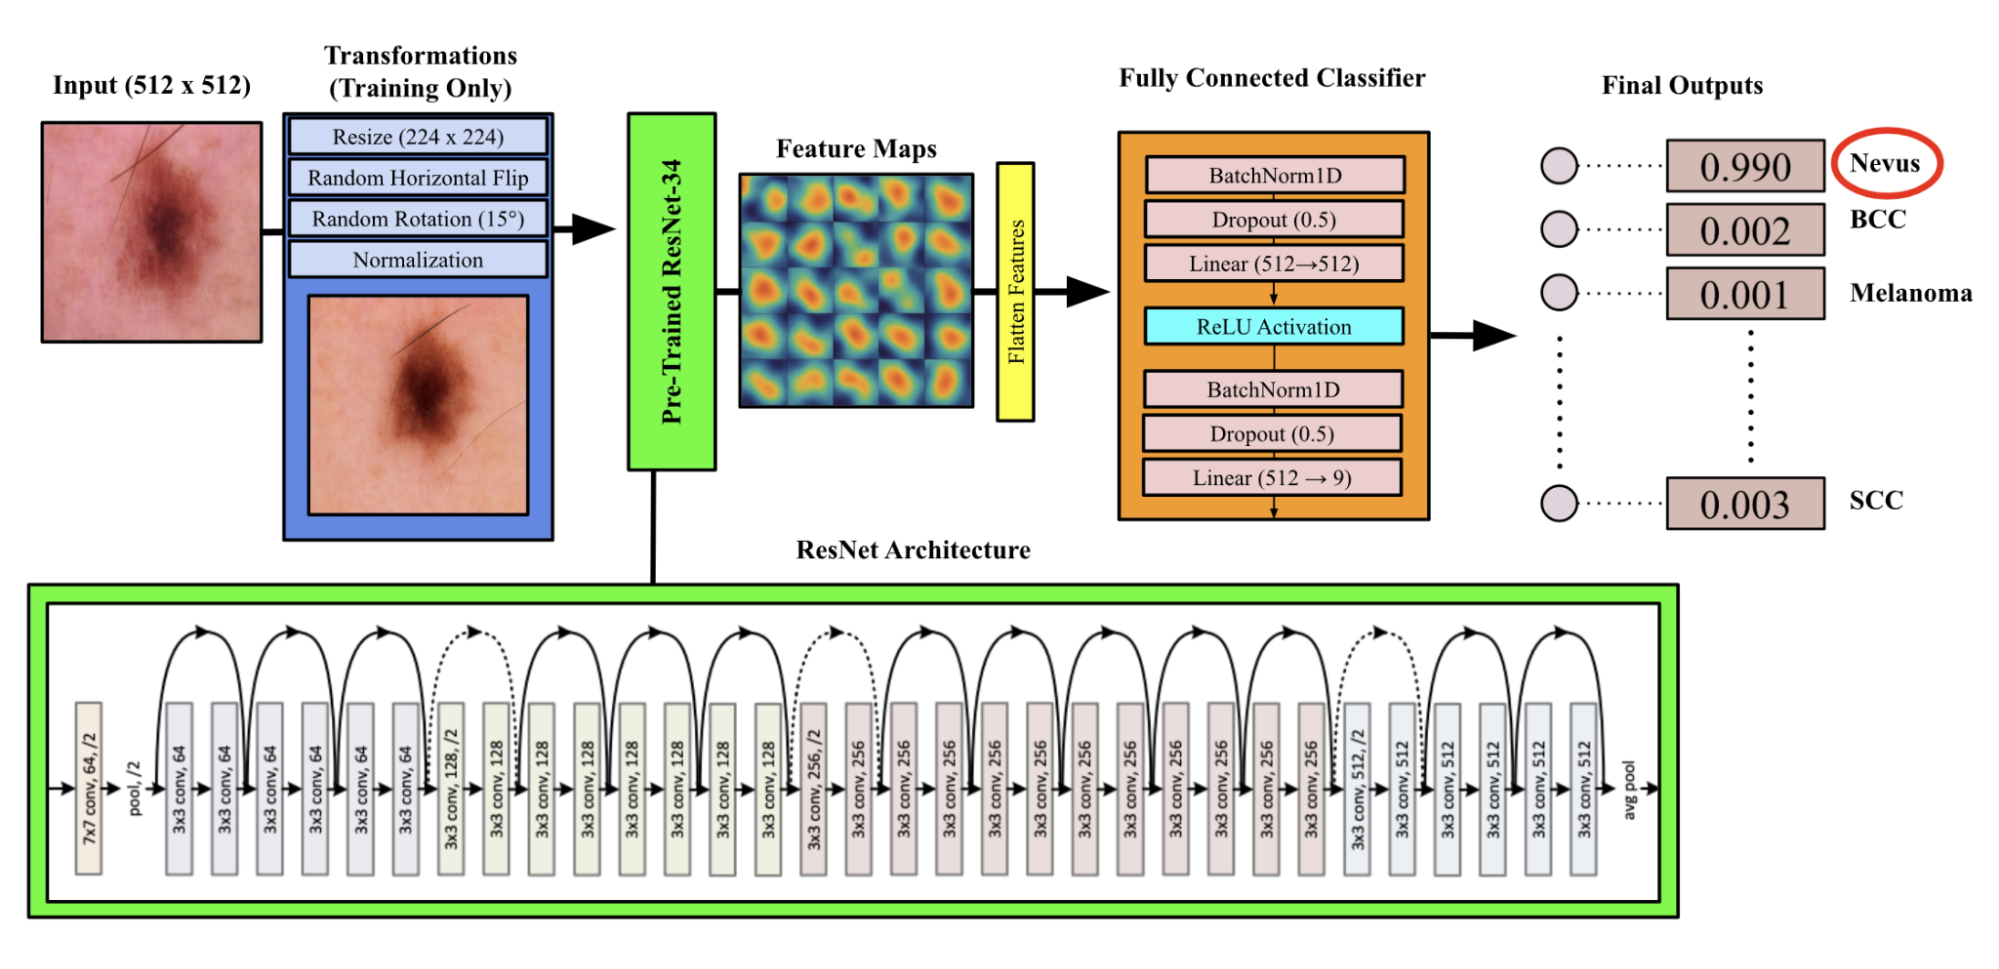
\includegraphics[width=0.7\textwidth]{Figs/model_architecture.png}
\end{center}
\caption{Architecture of the best-performing model. The model uses a ResNet-34 convolutional backbone as a feature extractor, followed by a custom two-layer fully connected classifier. ResNet-34 includes multiple convolutional blocks with residual connections and average pooling. Data transformations are applied to input images during training to improve generalization.}
\end{figure}

Currently, our best performing classifier exhibits a validation accuracy of 81.95\%, precision of 79.82\%, recall of 71.34\%, and F1 of 74.91\%. This model outperforms the baseline model and may still improve with further training. This model leverages a pre-trained ResNet-34 backbone for feature extraction, followed by a two-layer fully connected classifier. The classifier includes ReLU activation between the layers and applies batch normalization and dropout (with a rate of 0.5) before each linear transformation. The first linear layer receives the flattened output features from the ResNet-34 and projects them into a 512-dimensional hidden space. The final linear layer maps these features to 9 output units, corresponding to the number of skin lesion classes.


\begin{table}[h]
\caption{Best model hyperparameter values}
\label{hyperparameters}
\begin{center}
\footnotesize
\begin{tabularx}{\textwidth}{lXl}
\toprule
\textbf{Hyperparameter} & \textbf{Value} & \textbf{Description} \\
\midrule
NUM\_CLASSES & 9 & Number of output classes \\
BATCH\_SIZE & 64 & Samples per training batch \\
EPOCHS & 60 & Maximum training epochs \\
LEARNING\_RATE & 0.0003 & Initial learning rate \\
PATIENCE & 10 & Epochs to wait before early stopping \\
WEIGHT\_DECAY & 1e-4 & L2 regularization strength \\
LABEL\_SMOOTHING & 0.1 & Softens target labels to reduce overconfidence \\
BACKBONE & ResNet34 (pretrained) & CNN used for feature extraction \\
DROPOUT\_RATES & 0.5 (applied twice) & Dropout to reduce overfitting in classifier head \\
HIDDEN\_LAYER\_UNITS & 512 & Units in intermediate fully connected layer \\
IMAGE\_SIZE & 224 × 224 & Input image resolution \\
AUGMENTATIONS & Flip, Rotation & Data augmentation for robustness \\
NORMALIZATION\_MEAN & [0.485, 0.456, 0.406] & Standard normalization mean \\
NORMALIZATION\_STD & [0.229, 0.224, 0.225] & Standard normalization std dev \\
SAMPLER & WeightedRandomSampler & Balances class frequencies during training \\
SCHEDULER & ReduceLROnPlateau (factor=0.5) & Reduces LR when validation accuracy plateaus \\
OPTIMIZER & Adam & Optimizer used \\
CRITERION & CrossEntropyLoss (smoothing=0.1) & Loss function used \\
\bottomrule
\end{tabularx}
\end{center}
\end{table}

\begin{figure}[h]
\begin{center}
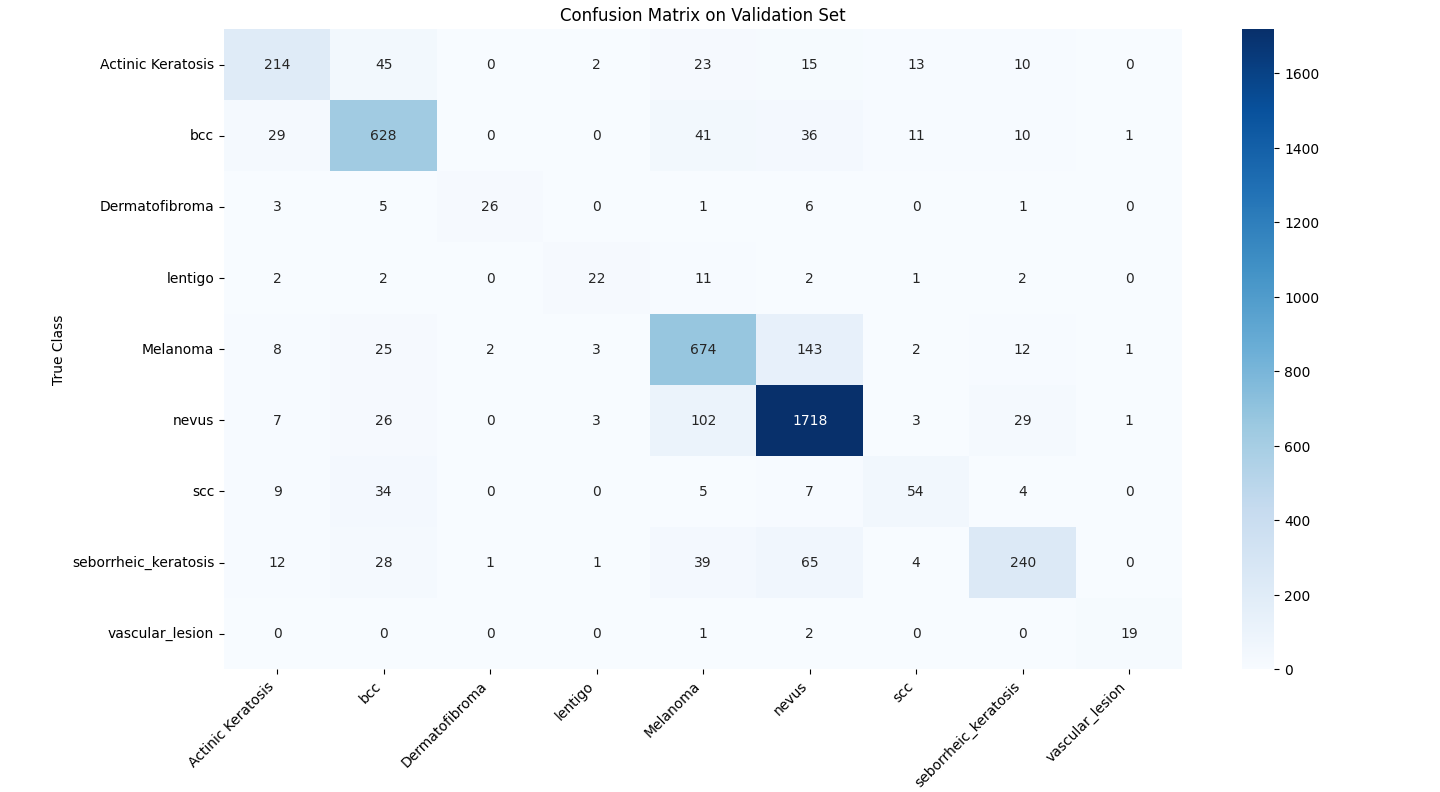
\includegraphics[width=1.0\textwidth]{Figs/confusion_matrix.png}
\end{center}
\caption{Confusion matrix of best model. The model predicts most classes effectively. However, it continues to confuse melanoma with nevus, actinic keratosis with BCC, and seborrheic keratosis with nevus, and SCC with BCC. In general, the model must reduce the chance of dangerous conditions like melanoma from being misclassified as benign conditions like nevi.}
\end{figure}

\begin{figure}[h]
\begin{center}
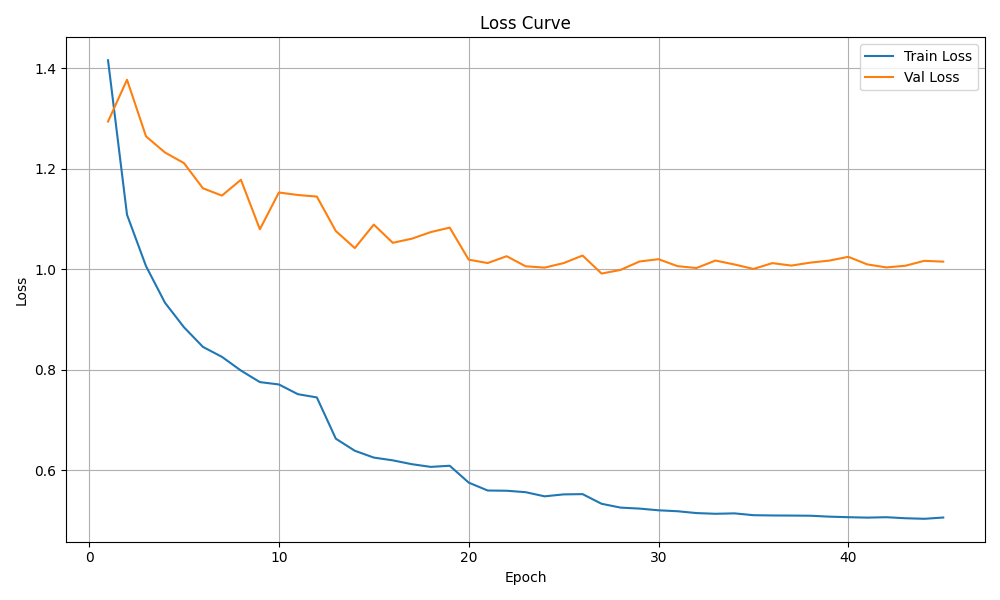
\includegraphics[width=0.7\textwidth]{Figs/training_validation_loss.png}
\end{center}
\caption{Best model validation and training loss per epoch. Train loss is steadily lower than validation loss due to the effects of WeightedRandomSampler, which makes the class distribution seen by the model in training different than in validation.}
\end{figure}

The 512 × 512 images were resized and augmented to 224 × 224 images with random rotations and reflections to reduce model complexity. The model is trained using the Adam optimizer with an initial learning rate of 0.0003 and a weight decay of 0.0001. Cross-entropy loss with label smoothing ($\varepsilon$ = 0.1) is used to prevent overconfident predictions. A learning rate scheduler (ReduceLROnPlateau) monitors validation accuracy and reduces the learning rate by a factor of 0.5 if no improvement is seen for 2 consecutive epochs. We trained our model for 45 epochs using early stopping with patience of 10 epochs. Due to the data imbalance, precision, recall, and F1 score were measured in addition to loss and accuracy.

\begin{figure}[h]
\begin{center}
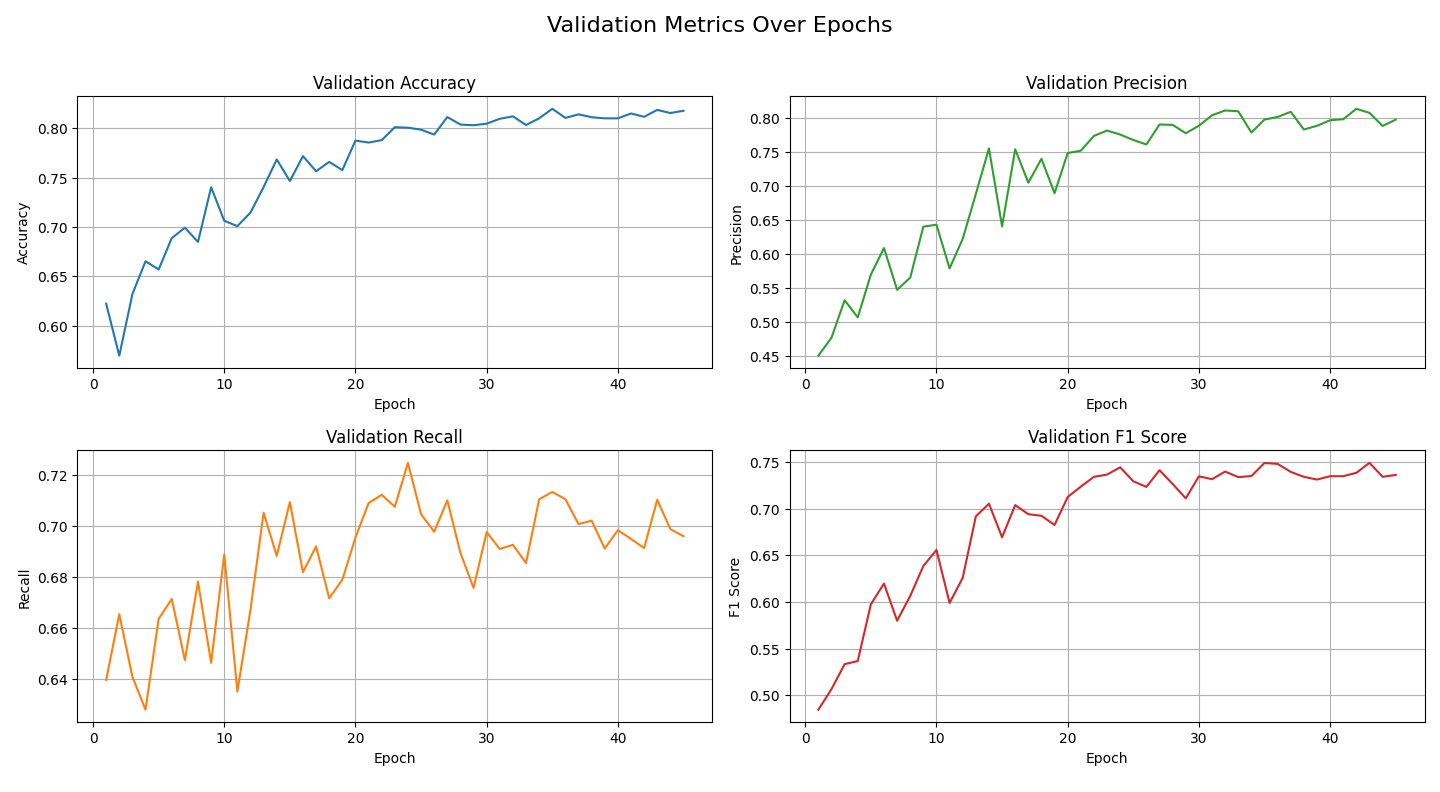
\includegraphics[width=0.8\textwidth]{Figs/validation_metrics.png}
\end{center}
\caption{Best model validation accuracy, precision, recall, and F1 per epoch. Validation metrics plateau after epoch 35.}
\end{figure}

\subsubsection{Challenges}

Each major training challenge and some proposed or implemented solution(s) are listed below.

\textbf{1. Dataset imbalance}

The imbalance of our combined dataset led our initial models to overpredict majority classes like nevi and melanoma and ignore minority classes like vascular lesion. The models exhibited high accuracy but low recall and precision, indicating poor generalization. To address the effects of dataset imbalance, we applied WeightedRandomSampler in training to sample classes inversely proportional to their frequency in the training dataset. This step balances each batch seen by the model during training so the model does not learn to predict only the majority class. Additionally, we randomly augmented images using random rotation and horizontal flipping, allowing the model to train on more unique minority class images.

\textbf{2. GPU Usage and Training Time}

To train our model we used a NVIDIA GeForce RTX 4050 GPU with a VRAM of 6 GB. Using 512 × 512 images and training large feature extractors like ResNet-50 and MobileNet required small batch sizes or was infeasible given our time frame. To increase training speed and feasibility, we resized the images to 224 × 224 before input into the model and unfroze only the last several layers in the feature extractors or opted for less complicated models. For example, our best model used ResNet-34 instead of the more complicated ResNet-50. This step also allowed us to use a batch size of 64 rather than 32 or 16 to smoothen training.

\textbf{3. Overfitting to Training Data}

Training on larger models like ResNet-50 led to sharp declines in training loss with little plateauing validation loss, indicating overfitting. To prevent overfitting, we applied two dropout layers of 0.5 to prevent the model from relying too heavily on specific neural pathways, used the smaller ResNet-34 and froze layers to reduce model size, and weight decay of 0.0001 to prevent overreliance on large weights. Data augmentation of the training set also reduced overfitting by preventing the model from memorizing images in their default orientations.

\label{last_page}

\bibliography{APS360_ref}
\bibliographystyle{iclr2022_conference}

\end{document}
